% Ajustar esse \vspace de acordo com o necessário
\vspace{-42pt}
\section[Automatização de processos]{Automatização de processos}
Automatizar processos significa passar as tarefas realizadas de maneira manual pelas pessoas para equipamentos, máquinas, instrumentos e outros \cite{AutomatProcess}. Para que a automatização de processos ofereça os resultados esperados, é muito importante garantir que sua implantação seja feita de maneira estruturada e de acordo com as diretrizes de onde está sendo aplicado \cite{AutomatProcess2}.No meio industrial, a preocupação com produtividade, redução do risco operacional e qualidade, leva à implantação de sistemas de automatização. 

A parte operacional na automação industrial é uma parte do sistema que atua diretamente no processo e é um conjunto de elementos que fazem com que a máquina se mova e realize a operação desejada \cite{AutomatProcess3}, aperfeiçoamento constante das atividades dos processos.

Automação em processos indutrias foram abordadas nas disciplinas de Controle Inteligente e Sistemas Realimentados, onde eram abordados diversos meios de controlar o processo. Neste projeto desenvolverá principalmente um sistema de software e hardware para automatizar o processo de emprétimos de equipamentos do laboratório.

\section[Aplicação WEB]{Aplicação WEB}
uma aplicação web é um software que é instalado em um servidor web e é projetado para responder a solicitações, processar informações, armazenar informações e dimensionar as respostas de acordo com a demanda e, em muitos casos, é distribuído em vários sistemas ou servidores \cite{WEB1}. Essas aplicações apresenta várias linguagens de programação (PHP, Javascript, etc) e elementos de interface gráfica (HTML, CSS).

As aplicações web se diferenciam das aplicações ‘desktop’ pois não precisa de instalação no computador, acessíveis de qualquer lugar com Internet, não depende de sistema operacional tendo todo o processamento de funções e instruções feito no servidor web e o navegador funciona apenas como uma ‘interface’ da  aplicação \cite{WEB2}. Essas vantagens de aplicação WEB foram vistas principalmente na displina  Redes de Computadores e de Automação.

Há a existencia de frameworks. Um framework em desenvolvimento de software, é uma abstração que une códigos comuns entre vários projetos de software provendo uma funcionalidade genérica \cite{WEB3}. Assim teremos para o desenvolvimento para esse software a framework chamada CakePHP \cite{Cake} que  torna a construção de aplicativos da web mais simples, mais rápida e requer menos código. 

\section[Banco de Dados]{Banco de Dados}
Um banco de dados é uma coleção de dados inter-relacionados, representando informações sobre um domínio específico, ou seja, sempre que for possível agrupar informações que se relacionam e tratam de um mesmo assunto, posso dizer que tenho um banco de dados \cite{BD1}. Como exemplo de banco de dados podemos citar um sistema de bibliotecas, uma agenda telefônica, um cadastro de clientes, etc.

Um sistema de gerenciamento de banco de dados (SGBD) é um software que possui recursos capazes de manipular as informações do banco de dados e interagir com o usuário. Existem vários SGBD’s no mercado, como Oracle, SQL Server, DB2, PostgreSQL, MySQL, o próprio Access ou Paradox, entre outros \cite{BD1}.

Os sistemas de banco de dados têm certas vantagens em relação ao sistema tradicional de armazenamento de arquivos. Eles são implementados com a função de isolar os detalhes internos do banco de dados do usuário, ou seja, promover a abstração desses dados e também permitir a relativa dependência dos dados e aplicativos que acessam \cite{BD1}.

Outro fator importante é a questão da segurança e integridade dos dados, pois estes são geralmente criptografados e não são acessados tão facilmente. No entanto, a implantação de um sistema de banco de dados é mais cara e nem sempre é necessário usá-lo \cite{BD1}.

Para realizar consultas, inserir, editar e vincular dados armazenados no banco de dados, é usada uma linguagem baseada em consultas estruturadas chamada SQL (Structured Query Language) \cite{BD1}.

A importancia em banco de dados foi abordado principalmente em disciplinas como Controle Inteligente. O banco de dados será  utilizado para armazenar os dados do empréstimos de equipamentos. SGBD utilizado será o MySQL, devido o fato de estar presente no XAMPP, que é um pacote com os principais servidores de código aberto do mercado, utilizado para o desenvolvimento da interface WEB \cite{BD2}.

Pode-se ser utilizado o modelo de banco de dados para o projeto para o projeto dado pela figura \ref{fig:ConfiBanco}.

\begin{figure}[!h]
	\centering
	\caption{Configuração do Banco de Dados.}
	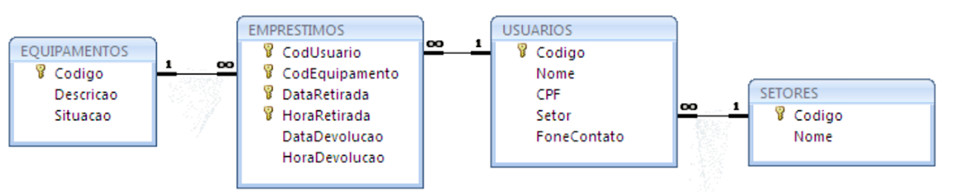
\includegraphics[width=0.7\textwidth]{figura4.jpg}
	\source[\citeonline{SistBib}.]
	\label{fig:ConfiBanco}
\end{figure}

Na figura \ref{fig:ConfiBanco2} apresenta outra forma de configuração do BD.

\begin{figure}[!h]
	\centering
	\caption{Outra configuração de Banco de dados}
	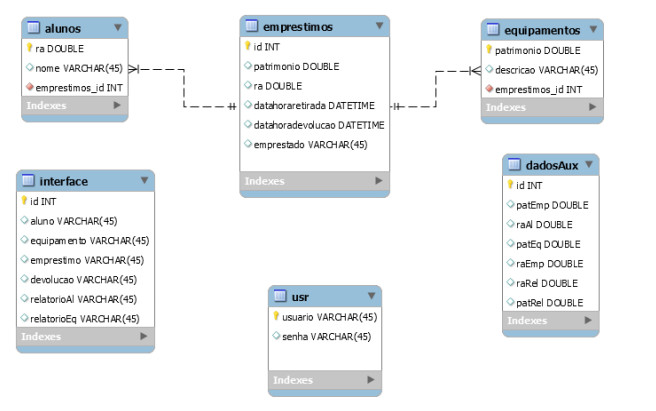
\includegraphics[width=0.7\textwidth]{figura7.jpg}
	\source[\citeonline{TCC}.]
	\label{fig:ConfigBanco2}
\end{figure}


Na figura \ref{fig:BancoAcess} mostra um esquemático de como vai ser acessado o banco de dados.

\begin{figure}[!h]
	\centering
	\caption{Acesso do Banco de Dados.}
	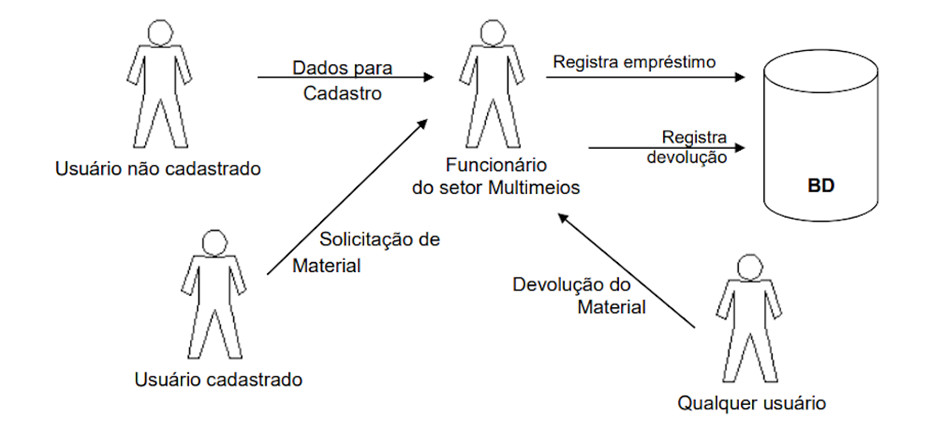
\includegraphics[width=0.7\textwidth]{figura5.jpg}
	\source[\citeonline{SistBib}.]
	\label{fig:BancoAcess}
\end{figure}


\section[Sistema Embarcado]{Sistema Embarcado}

O sistema embarcado, também chamado de sistema embutido, é um sistema microprocessado em que um computador está anexado ao sistema que ele controla. Um sistema embarcado pode realizar um conjunto de tarefas que foram predefinidas. O sistema é usado para tarefas específicas, e assim, através de engenharia é possível otimizar um determinado produto e diminuir o tamanho, bem como os recursos computacionais e o seu valor final \cite{embarcado}.

Os sistemas embarcados estão por toda a nossa volta, e por essa razão, não nos damos conta de sua capacidade computacional, já que estamos tão envolvidos com tais mecanismos \cite{embarcado}. Há uma grande variedade de processadores disponíveis no mercado, o que leva ao desevolviemento de vários sistemas.

Há muitas restrições em sistemas embarcados comparando com os computadores convensionais. Entre eles, as restrições dimensionais, que envolvem tamanho e peso, são extremamente importantes em equipamentos pequenos, como telefones celulares. Outra restrição é o consumo de energia, que é extremamente importante em equipamentos móveis e é alimentado por baterias, como no caso de um dispositivo GPS. Restrições de recursos, como memória e processamento, afetam o design do software. Deve ter um software eficaz para que seu sistema não enfrente problemas. Outra restrição que pode ser citada é a da execução. Isso é relevante porque vários aplicativos devem ser executados em um momento muito específico.

O sistema embarcado é dedicado a uma única finalidade, ou um pequeno conjunto de propósitos \cite{embarcado2}. Ele é depende da sua aplicação. 

Sistemas Embarcados foi abordado nas disciplinas como Sistemas Embarcados, Eletrônica Básica 1 e 2. Será utilizado este conceito para desenvolver um sistema que tenha o sistema que irá informar a localização do equipamento e também o sistema que irá reconhecer o código do equipamento e a matrícula do aluno através do código de barras quando for ser feito o emprétimo. 
